Nesta seção explicamos as duas integrações que fizemos com exercícios-programas dados em disciplinas de introdução a computação e que envolviam física.

\subsection{Configuração}
\subsection{Angry Bixos}

\begin{figure}[H]
    \centering
	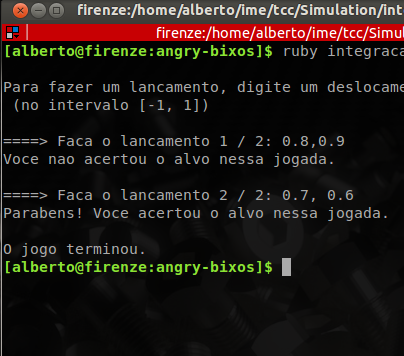
\includegraphics[scale=0.6]{images/angry-bixos-3.png}
	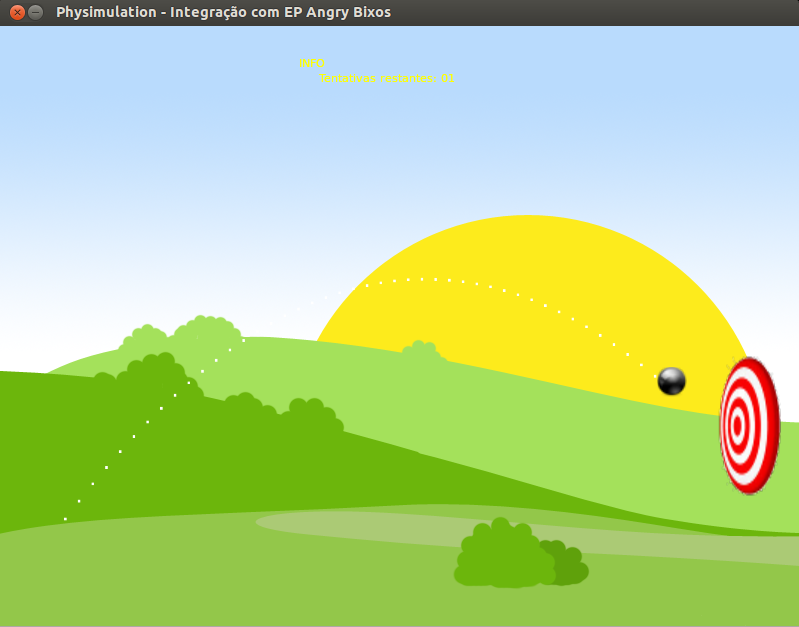
\includegraphics[scale=0.22]{images/angry-bixos-4.png}
	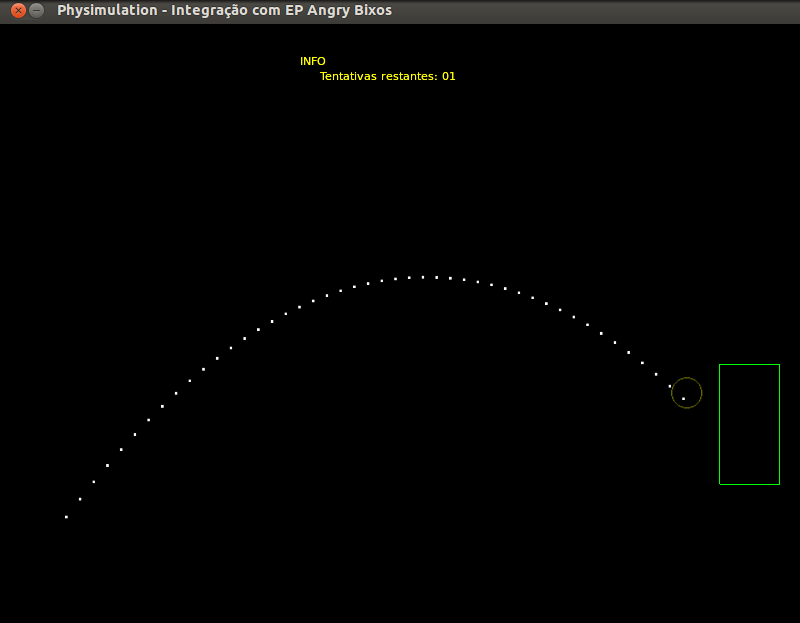
\includegraphics[scale=0.22]{images/angry-bixos-4E.png}
	\caption{Integração com EP Angry Bixos}
\end{figure}

\subsection{Apolo}

\begin{figure}[H]
    \centering
	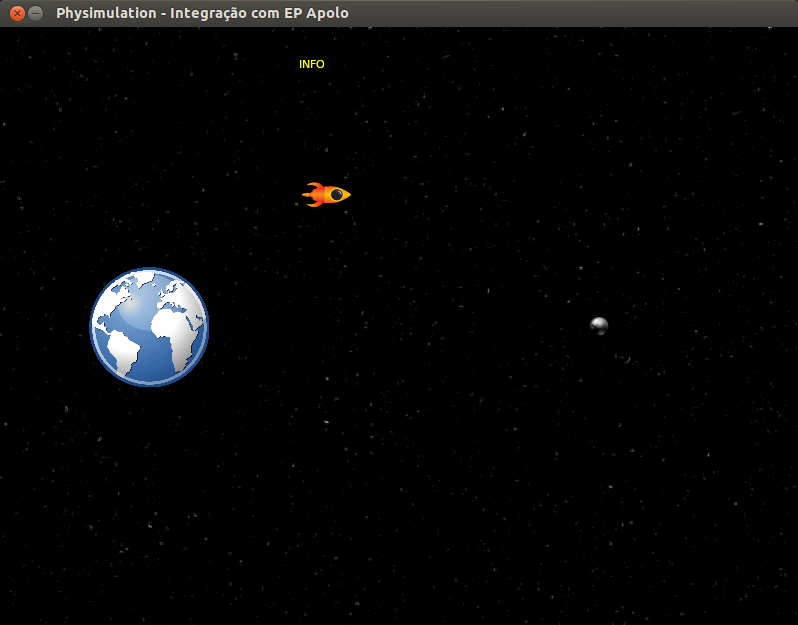
\includegraphics[scale=0.22]{images/apolo-4.png}
	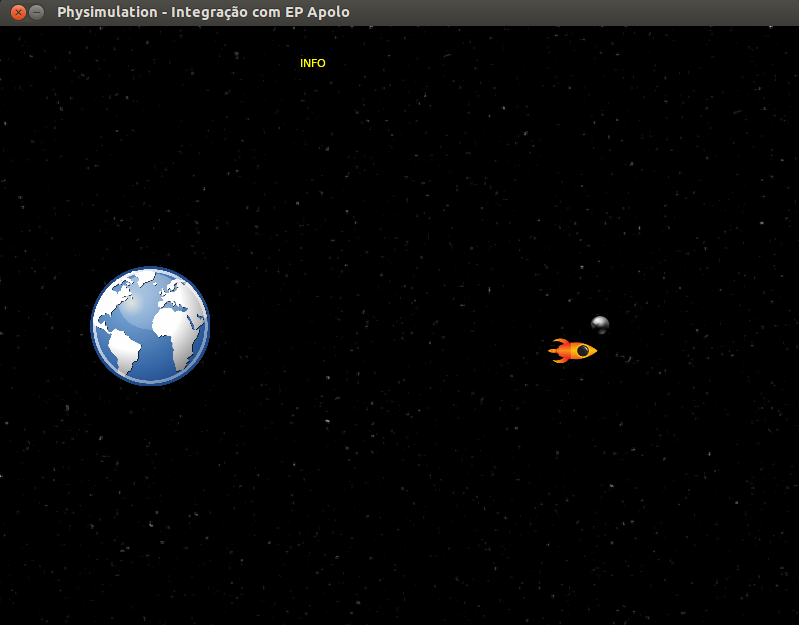
\includegraphics[scale=0.22]{images/apolo-6.png}
	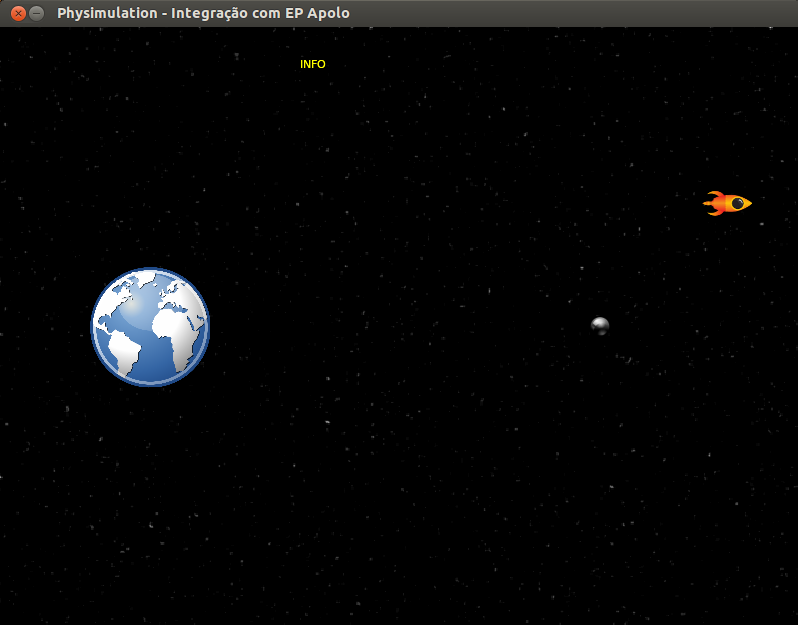
\includegraphics[scale=0.22]{images/apolo-3.png}
	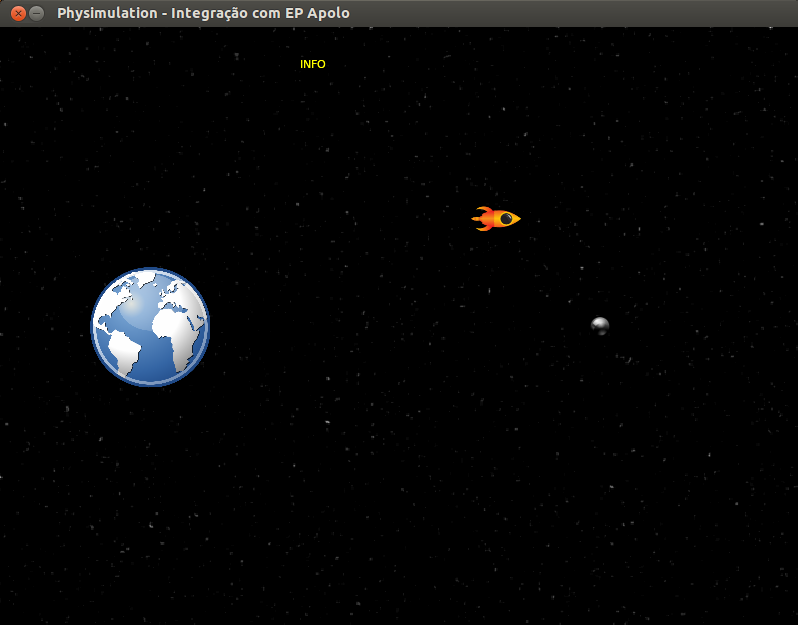
\includegraphics[scale=0.22]{images/apolo-2.png}
	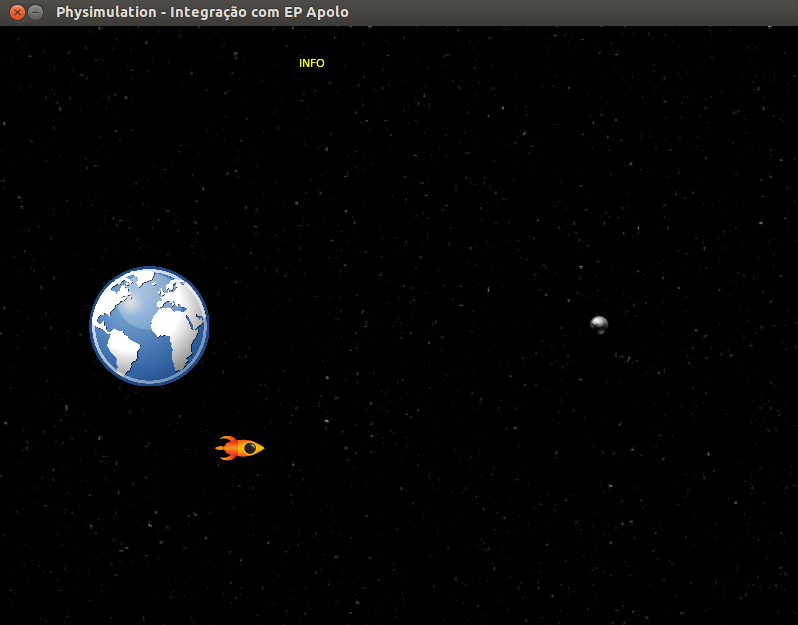
\includegraphics[scale=0.22]{images/apolo-1.png}
	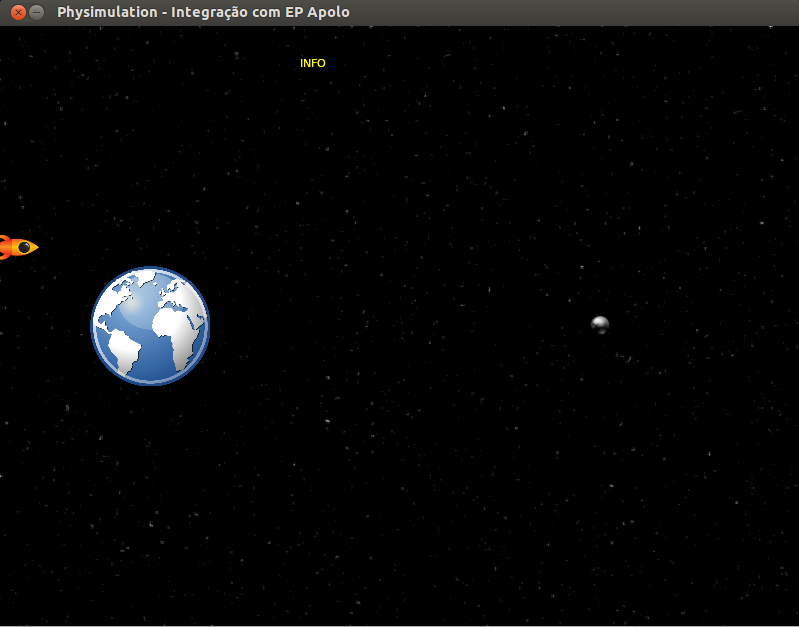
\includegraphics[scale=0.22]{images/apolo-5.png}
	\caption{Efeito \textit{slingshot} Integração com EP Apolo}
\end{figure}


